% ============================================================================
%  Ideal Chemistry Manuscript Template (LaTeX)
%  Part of ideal-chemistry-academic-writing
%  Journal-agnostic skeleton: satisfies ACS / RSC / Wiley structural norms.
%  Compile:  pdflatex main.tex && bibtex main && pdflatex main.tex && pdflatex main.tex
% ============================================================================
\documentclass[12pt,a4paper]{article}

% --- Language & encoding ---
\usepackage[utf8]{inputenc}
\usepackage[T1]{fontenc}
\usepackage{newtxtext,newtxmath}   % Times-like: closest to journal house style
\usepackage{microtype}

% --- Chemistry ---
\usepackage[version=4]{mhchem}     % \ce{...} for chemical equations
\usepackage{chemfig}               % structures
\usepackage{chemmacros}            % \ce{}, \pKa etc. (optional)

% --- Layout ---
\usepackage[a4paper,left=2.5cm,right=2.5cm,top=2.5cm,bottom=2.5cm]{geometry}
\usepackage{setspace}
\onehalfspacing                    % journals ask 1.5 or double for review copies
\usepackage{graphicx}
\graphicspath{{figures/}}
\usepackage{booktabs,array,multirow}
\usepackage{siunitx}               % \SI{3.2}{\milli\molar}, \num{1.2e5}
\usepackage[font=small,labelfont=bf]{caption}
\usepackage[colorlinks=true,linkcolor=blue,citecolor=blue,urlcolor=blue]{hyperref}

% --- Manuscript control ---
\usepackage{xcolor}
\newcommand{\change}[1]{\textcolor{blue}{#1}}   % mark revisions in blue
\usepackage{lineno}
\linenumbers                              % required by many journals for review

% --- References: numbered (ACS-like). Alternatives available in TeX Live:
%   \usepackage[round,authoryear]{natbib} + \bibliographystyle{rsc}      % RSC author-year
%   \bibliographystyle{angew}                                            % Wiley/Angew (numbered)
%   For true ACS style, use the official achemso class (github.com/josephwright/achemso).
\usepackage[numbers,sort&compress]{natbib}
\bibliographystyle{unsrtnat}

\title{\bfseries Title: Informative, $\le$18 words, No Hype Words}
\author{First Author,\textsuperscript{a} Second Author,\textsuperscript{a} Corresponding Author,\textsuperscript{a,*}\\
  \textsuperscript{a}Department of Chemistry, Indian Institute of Science Education and
  Research Bhopal, Bhopal Bypass Road, Bhauri, Bhopal 462066, Madhya Pradesh, India.\\
  *E-mail: corresponding@iiserb.ac.in}
\date{}

\begin{document}

\maketitle
\thispagestyle{empty}

% ---------------------------------------------------------------------------
% ABSTRACT  (ACS: <=300 words Articles / <=150 Letters; RSC: 50-250; Wiley: <=200)
% Four moves: context -> gap/approach -> key results (quantitative) -> impact.
% No references, no graphics, no compound numbers.
% ---------------------------------------------------------------------------
\begin{abstract}
\noindent The problem and why it matters (1--2 sentences). What was missing and
what we did (1--2 sentences). Key results with numbers: yield \SI{82}{\percent},
rate constant $k=\SI{3.4(2)e-3}{\per\second}$, detection limit
\SI{48}{\nano\molar} (2--4 sentences). What it means for the field (1 sentence).
\end{abstract}

\noindent\textbf{Keywords:} keyword one; keyword two; keyword three; keyword four;
keyword five

% ---------------------------------------------------------------------------
% TOC / GRAPHICAL ABSTRACT — required by ACS (3.25 x 1.75 in), RSC (8 x 4 cm),
% Wiley (5.5 x 5.0 cm).  Generate one at the exact pixel size with:
%   paperforge scheme toc "reactant>>product" --journal "Organic Letters" --out toc.png
% ---------------------------------------------------------------------------
\begin{center}
\fbox{\parbox[c][4.45cm][c]{8.25cm}{\centering TOC graphic placeholder\\
\normalsize ACS 8.25 $\times$ 4.45 cm \\ (Chem. Commun.\ 8 $\times$ 4 cm; Angew.\ 5.5 $\times$ 5 cm)}}
\end{center}

% ---------------------------------------------------------------------------
% 1. INTRODUCTION
% ---------------------------------------------------------------------------
\section{Introduction}
\label{sec:intro}

Field-level context, not textbook background \citep{romero2016organic}. State of
the art with key primary references \citep{xin2026recent,yang2023recent}.
The gap: \emph{However, \ldots{} remains unexplored / suffers from limited scope /
lacks mechanistic understanding.}

Here we report \ldots{} (approach + headline result). This work demonstrates
\ldots{} (significance, one sentence).

% ---------------------------------------------------------------------------
% 2. RESULTS AND DISCUSSION
% ---------------------------------------------------------------------------
\section{Results and Discussion}
\label{sec:results}

\subsection{Synthesis and characterisation}
\label{sec:synthesis}

Scheme~\ref{sch:main} summarises the synthetic route. Compound \textbf{1} was
prepared according to the literature procedure \citep{pan2024base}, while
compounds \textbf{2}--\textbf{7} are new.

\begin{scheme}[htbp]
\centering
\schemestart
\chemfig{*6(-(-[::30]O-[::-30](-[::-60])=[::60]O)=-=(-OH)=-=-)}
\arrow{->[cat., solvent, T][yield \SI{82}{\percent}]}
\chemfig{*6(-(-[::30]O-[::-30](-[::-60])=[::60]O)=-=(-[::30]O-[::-30]([::60]R))=-=)}
\schemestop
\caption{Reaction scheme with conditions and yields.}
\label{sch:main}
\end{scheme}

Figure~\ref{fig:key} shows the key experimental result. The data reveal
\ldots{} (\SI{}{\micro\molar}, $\lambda_{\max} = \SI{452}{\nano\meter}$,
$\Phi_{\mathrm{PL}} = 0.31$).

\begin{figure}[htbp]
\centering
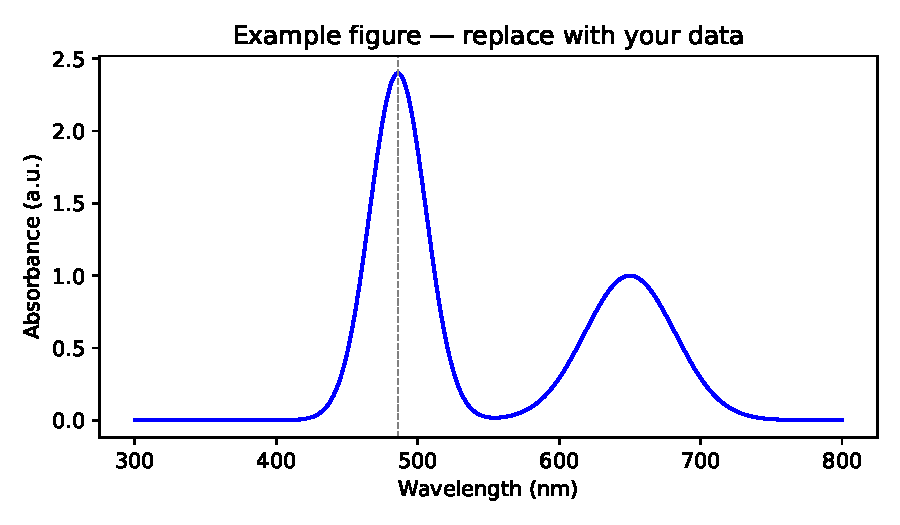
\includegraphics[width=0.85\linewidth]{example_figure.pdf}
\caption{Key figure: caption states what is shown, conditions, and the take-away.
Error bars shown where applicable.}
\label{fig:key}
\end{figure}

\subsection{Mechanistic investigation}
\label{sec:mechanism}

Control experiments (Table~\ref{tab:controls}) exclude \ldots{}. DFT calculations
at the \texttt{PBE0-D3BJ/def2-TZVP} level support \ldots{} (computational details:
software version, basis set, solvation model --- see SI).

\begin{table}[htbp]
\centering
\caption{Control experiments.}
\label{tab:controls}
\begin{tabular}{llcc}
\toprule
Entry & Variation & Yield (\%) & Conv. (\%) \\
\midrule
1 & standard conditions & 82 & >99 \\
2 & without catalyst & 0 & 5 \\
3 & without light & 12 & 18 \\
4 & with TEMPO (1.2 equiv.) & 0 & 3 \\
\bottomrule
\end{tabular}
\end{table}

% ---------------------------------------------------------------------------
% 3. CONCLUSION
% ---------------------------------------------------------------------------
\section{Conclusion}
\label{sec:conclusion}

We have shown that \ldots{} (2--4 sentences, data-backed, no new data). The results
open the way for \ldots{} (future directions, 1 sentence).

% ---------------------------------------------------------------------------
% 4. EXPERIMENTAL SECTION
% ---------------------------------------------------------------------------
\section{Experimental Section}
\label{sec:experimental}

\subsection{General methods}
\label{sec:genmethods}
All reagents were used as received unless otherwise stated. NMR spectra were
recorded on a Bruker Avance \SI{400}{\mega\hertz} spectrometer; chemical shifts
($\delta$) are in ppm relative to TMS ($\ce{^1H}$, $\ce{^{13}C}$). High-resolution
mass spectra were obtained on a Bruker microTOF-Q II (ESI). UV--vis spectra were
recorded on a Shimadzu UV-2600. \textbf{Safety:} all reactions with [hazardous
reagent] were performed in a fume hood behind a blast shield; no unexpected
hazards were encountered.

\subsection{General procedure for the synthesis of 2--7}
\label{sec:genproc}
A flame-dried Schlenk tube was charged with \textbf{1} (\SI{1.00}{\milli\mol},
\SI{0.212}{\gram}), [catalyst] (\SI{5}{\mol\percent}), and dry THF
(\SI{5}{\milli\liter}) under $\ce{N2}$. The mixture was stirred at
\SI{60}{\celsius} for 12 h. After cooling, the solvent was removed and the residue
purified by column chromatography (hexane/EtOAc, 9:1) to afford \textbf{2} as a
yellow solid.

\subsection{Characterisation data}
\label{sec:char}
% VERIFIED TEMPLATE DATA — every number below is internally consistent:
%   C14H11NO2S, MW 257.31, monoisotopic 257.0510, [M+H]+ 258.0583, DBE 10
%   1.00 mmol scale, 82% -> 0.82 mmol -> 0.211 g
%   1H integrals sum to 11 H (matches the formula)
% Replace with your own data, then run:  paperforge check <your project>
\textbf{2:} yield \SI{82}{\percent} (\SI{0.82}{\milli\mol}, \SI{0.211}{\gram});
yellow solid; mp \SIrange{142}{144}{\celsius}. \ce{^1H} NMR (\SI{400}{\mega\hertz},
\ce{CDCl3}) $\delta$ 8.21 (d, $J = \SI{8.8}{\hertz}$, 2H, ArH), 7.42 (dd,
$J = \SI{8.8}{\hertz}$ and \SI{2.1}{\hertz}, 2H, ArH), 6.98 (d, $J = \SI{2.1}{\hertz}$, 1H, ArH),
4.10 (q, $J = \SI{7.1}{\hertz}$, 2H, \ce{OCH2}), 3.92 (s, 3H, \ce{OCH3}),
1.28 (t, $J = \SI{7.1}{\hertz}$, 3H, \ce{CH3});
\ce{^{13}C}\{\ce{^1H}\} NMR (\SI{100}{\mega\hertz}, \ce{CDCl3}) $\delta$ 161.2,
158.9, 144.3, 131.8, 125.4, 120.7, 111.9, 66.4, 55.6, 14.3;
IR (KBr) $\tilde{\nu}$ 2224 (\ce{C#N}), 1608, 1512 cm$^{-1}$;
HRMS (ESI-TOF) $m/z$ calcd for \ce{C14H11NO2S} [M+H]$^{+}$ 258.0583, found 258.0587;
elemental analysis calcd for \ce{C14H11NO2S}: C 65.35, H 4.31, N 5.44; found C 65.31, H 4.29, N 5.47.

% Crystallographic statement (if applicable):
% CCDC 2400000 contains the supplementary crystallographic data for compound 4.
% These data can be obtained free of charge from the Cambridge Crystallographic
% Data Centre.

% ---------------------------------------------------------------------------
% SUPPORTING INFORMATION PARAGRAPH (ACS format)
% ---------------------------------------------------------------------------
\paragraph{Supporting Information.}
General experimental details, NMR spectra for compounds \textbf{2}--\textbf{7}
(PDF); HRMS spectra (PDF); crystallographic data for \textbf{4} (CIF);
DFT-optimised coordinates (XYZ); \ce{^1H} and \ce{^{13}C} NMR spectra for all new compounds (PDF).

\paragraph{Acknowledgements.}
This work was supported by [Agency] (Grant No. \ldots{}). We thank the Central
Instrumentation Facility, IISER Bhopal, for NMR and HRMS access.

\paragraph{Conflict of interest.}
The authors declare no competing financial interest.

\paragraph{Data availability.}
All data supporting this study are included in the paper and its Supporting
Information. Crystallographic data: CCDC 2400000--2400002. Computational
coordinates: Zenodo DOI 10.5281/zenodo.0000000.

\paragraph{CRediT authorship contribution statement.}
Author A: conceptualisation, investigation, writing -- original draft.
Author B: investigation, formal analysis. Author C: conceptualisation,
supervision, writing -- review \& editing.

% ---------------------------------------------------------------------------
% REFERENCES
% ---------------------------------------------------------------------------
\bibliography{refs}

\end{document}
